%% LyX 2.4.3 created this file.  For more info, see https://www.lyx.org/.
%% Do not edit unless you really know what you are doing.
\documentclass[journal,article,submit,pdftex,moreauthors]{Definitions/mdpi}
\usepackage{textcomp}
\usepackage[utf8]{inputenc}
\usepackage{float}
\usepackage{url}
\usepackage{varwidth}
\usepackage{graphicx}

\makeatletter

%%%%%%%%%%%%%%%%%%%%%%%%%%%%%% LyX specific LaTeX commands.

\Title{Classification of earthquakes using Grammatical Evolution}

\TitleCitation{Predicting the magnitude of earthquakes using Grammatical Evolution}

\Author{Constantina Kopitsa$^{1}$, Ioannis G. Tsoulos$^{2}$, Vasileios Charilogis$^{3}$
and Chrysostomos Stylios$^{4,*}$ }

\AuthorNames{Kopitsa, C., Tsoulos, I.G., Charilogs, V., Stylios C. }

\AuthorNames{Constantina Kopitsa, Ioannis G. Tsoulos, Vasileios Charilogis and
Chrysostomos Stylios}

\AuthorCitation{Kopitsa, C.; Tsoulos, I.G.; Charilogis, V.; Stylios, C. }


\address{$^{1}$\quad{}Department of Informatics and Telecommunications,
University of Ioannina, Greece;k.kopitsa@uoi.gr\\
$^{2}$\quad{}Department of Informatics and Telecommunications, University
of Ioannina, Greece; itsoulos@uoi.gr\\
$^{3}\quad$Department of Informatics and Telecommunications, University
of Ioannina, Greece; v.charilog@uoi.gr\\
$^{4}\quad$Department of Informatics and Telecommunications, University
of Ioannina, Greece; stylios@uoi.gr}


\corres{Correspondence: stylios@uoi.gr}


\abstract{Earthquake predictability remains a central challenge in seismology.
Are earthquakes inherently unpredictable phenomena, or can they be
forecasted through advances in technology? Contemporary seismological
research continues to pursue this scientific milestone, often referred
to as the ‘Holy Grail’ of earthquake prediction. In the direction
of earthquake prediction based on historical data, the Grammatical
Evolution technique of GenClass demonstrated high predictive accuracy
for earthquake magnitude. Similarly, our research team follows this
line of reasoning, operating under the belief that nature provides
a pattern that, with the appropriate tools, can be decoded. What is
certain is that, over the past 30 years, scientists and researchers
have made significant strides in the field of seismology, largely
aided by the development and application of artificial intelligence
techniques. Artificial Neural Networks (ANNs) were first applied in
the domain of seismology in 1994. The introduction of Deep Neural
Networks (DNNs), characterized by architectures incorporating two
hidden layers, followed in 2002. Subsequently, Recurrent Neural Networks
(RNNs) were implemented within seismological studies as early as 2007.
Most recently, Grammatical Evolution (GE) has been introduced in seismological
studies (2025). Despite continuous progress in the field, achieving
the so-called “triple prediction” --- the precise estimation of the
time, location, and magnitude of an earthquake --- remains elusive.
Nevertheless, machine learning and soft computing approaches have
long played a significant role in seismological research. Concerning
these approaches, significant advancements have been achieved, both
in mapping seismic patterns and in predicting seismic characteristics
on a smaller geographical scale. In such a way, our research will
analyze historical seismic events from 2004 to 2011, for the Latitude
21°-79° \& Longitude 33\textbf{°-}176°. The data will be categorized
and classified, with the aim of employing Grammatical Evolution techniques
to achieve more accurate and timely predictions of earthquake magnitudes.
This paper presents a systematic effort to enhance magnitude prediction
accuracy using GE, contributing to the broader goal of reliable earthquake
forecasting. Subsequently, in this paper we present the superiority
of GenClass, a key element of the Grammatical Evolution techniques,
with an average error of 19\%, indicating an overall accuracy of 81\%. }


\keyword{Earthquakes; Machine learning; Neural networks; Grammatical Evolution;}

\DeclareTextSymbolDefault{\textquotedbl}{T1}
%% Because html converters don't know tabularnewline
\providecommand{\tabularnewline}{\\}
%% Variable width box for table cells
\newenvironment{cellvarwidth}[1][t]
    {\begin{varwidth}[#1]{\linewidth}}
    {\@finalstrut\@arstrutbox\end{varwidth}}

%%%%%%%%%%%%%%%%%%%%%%%%%%%%%% User specified LaTeX commands.
%  LaTeX support: latex@mdpi.com 
%  For support, please attach all files needed for compiling as well as the log file, and specify your operating system, LaTeX version, and LaTeX editor.

%=================================================================
%\documentclass[preprints,article,submit,pdftex,moreauthors]{Definitions/mdpi} 
% For posting an early version of this manuscript as a preprint, you may use "preprints" as the journal. Changing "submit" to "accept" before posting will remove line numbers.

% Below journals will use APA reference format:
% admsci, aichem, behavsci, businesses, econometrics, economies, education, ejihpe, famsci, games, humans, ijcs, ijfs, journalmedia, jrfm, languages, psycholint, publications, tourismhosp, youth

% Below journals will use Chicago reference format:
% arts, genealogy, histories, humanities, jintelligence, laws, literature, religions, risks, socsci

%--------------------
% Class Options:
%--------------------
%----------
% journal
%----------
% Choose between the following MDPI journals:
% accountaudit, acoustics, actuators, addictions, adhesives, admsci, adolescents, aerobiology, aerospace, agriculture, agriengineering, agrochemicals, agronomy, ai, air, algorithms, allergies, alloys, amh, analytica, analytics, anatomia, anesthres, animals, antibiotics, antibodies, antioxidants, applbiosci, appliedchem, appliedmath, appliedphys, applmech, applmicrobiol, applnano, applsci, aquacj, architecture, arm, arthropoda, arts, asc, asi, astronomy, atmosphere, atoms, audiolres, automation, axioms, bacteria, batteries, bdcc, behavsci, beverages, biochem, bioengineering, biologics, biology, biomass, biomechanics, biomed, biomedicines, biomedinformatics, biomimetics, biomolecules, biophysica, biosensors, biosphere, biotech, birds, blockchains, bloods, blsf, brainsci, breath, buildings, businesses, cancers, carbon, cardiogenetics, catalysts, cells, ceramics, challenges, chemengineering, chemistry, chemosensors, chemproc, children, chips, cimb, civileng, cleantechnol, climate, clinbioenerg, clinpract, clockssleep, cmd, cmtr, coasts, coatings, colloids, colorants, commodities, complications, compounds, computation, computers, condensedmatter, conservation, constrmater, cosmetics, covid, crops, cryo, cryptography, crystals, csmf, ctn, curroncol, cyber, dairy, data, ddc, dentistry, dermato, dermatopathology, designs, devices, diabetology, diagnostics, dietetics, digital, disabilities, diseases, diversity, dna, drones, dynamics, earth, ebj, ecm, ecologies, econometrics, economies, education, eesp, ejihpe, electricity, electrochem, electronicmat, electronics, encyclopedia, endocrines, energies, eng, engproc, ent, entomology, entropy, environments, epidemiologia, epigenomes, esa, est, famsci, fermentation, fibers, fintech, fire, fishes, fluids, foods, forecasting, forensicsci, forests, fossstud, foundations, fractalfract, fuels, future, futureinternet, futureparasites, futurepharmacol, futurephys, futuretransp, galaxies, games, gases, gastroent, gastrointestdisord, gastronomy, gels, genealogy, genes, geographies, geohazards, geomatics, geometry, geosciences, geotechnics, geriatrics, glacies, grasses, greenhealth, gucdd, hardware, hazardousmatters, healthcare, hearts, hemato, hematolrep, heritage, higheredu, highthroughput, histories, horticulturae, hospitals, humanities, humans, hydrobiology, hydrogen, hydrology, hygiene, idr, iic, ijerph, ijfs, ijgi, ijmd, ijms, ijns, ijpb, ijt, ijtm, ijtpp, ime, immuno, informatics, information, infrastructures, inorganics, insects, instruments, inventions, iot, j, jal, jcdd, jcm, jcp, jcs, jcto, jdad, jdb, jeta, jfb, jfmk, jimaging, jintelligence, jlpea, jmahp, jmmp, jmms, jmp, jmse, jne, jnt, jof, joitmc, joma, jop, jor, journalmedia, jox, jpbi, jpm, jrfm, jsan, jtaer, jvd, jzbg, kidney, kidneydial, kinasesphosphatases, knowledge, labmed, laboratories, land, languages, laws, life, lights, limnolrev, lipidology, liquids, literature, livers, logics, logistics, lubricants, lymphatics, machines, macromol, magnetism, magnetochemistry, make, marinedrugs, materials, materproc, mathematics, mca, measurements, medicina, medicines, medsci, membranes, merits, metabolites, metals, meteorology, methane, metrics, metrology, micro, microarrays, microbiolres, microelectronics, micromachines, microorganisms, microplastics, microwave, minerals, mining, mmphys, modelling, molbank, molecules, mps, msf, mti, multimedia, muscles, nanoenergyadv, nanomanufacturing, nanomaterials, ncrna, ndt, network, neuroglia, neurolint, neurosci, nitrogen, notspecified, nursrep, nutraceuticals, nutrients, obesities, oceans, ohbm, onco, oncopathology, optics, oral, organics, organoids, osteology, oxygen, parasites, parasitologia, particles, pathogens, pathophysiology, pediatrrep, pets, pharmaceuticals, pharmaceutics, pharmacoepidemiology, pharmacy, philosophies, photochem, photonics, phycology, physchem, physics, physiologia, plants, plasma, platforms, pollutants, polymers, polysaccharides, populations, poultry, powders, preprints, proceedings, processes, prosthesis, proteomes, psf, psych, psychiatryint, psychoactives, psycholint, publications, purification, quantumrep, quaternary, qubs, radiation, reactions, realestate, receptors, recycling, regeneration, religions, remotesensing, reports, reprodmed, resources, rheumato, risks, robotics, rsee, ruminants, safety, sci, scipharm, sclerosis, seeds, sensors, separations, sexes, signals, sinusitis, siuj, skins, smartcities, sna, societies, socsci, software, soilsystems, solar, solids, spectroscj, sports, standards, stats, std, stresses, surfaces, surgeries, suschem, sustainability, symmetry, synbio, systems, tae, targets, taxonomy, technologies, telecom, test, textiles, thalassrep, therapeutics, thermo, timespace, tomography, tourismhosp, toxics, toxins, transplantology, transportation, traumacare, traumas, tropicalmed, universe, urbansci, uro, vaccines, vehicles, venereology, vetsci, vibration, virtualworlds, viruses, vision, waste, water, wem, wevj, wild, wind, women, world, youth, zoonoticdis

%---------
% article
%---------
% The default type of manuscript is "article", but can be replaced by: 
% abstract, addendum, article, book, bookreview, briefreport, casereport, comment, commentary, communication, conferenceproceedings, correction, conferencereport, entry, expressionofconcern, extendedabstract, datadescriptor, editorial, essay, erratum, hypothesis, interestingimage, obituary, opinion, projectreport, reply, retraction, review, perspective, protocol, shortnote, studyprotocol, systematicreview, supfile, technicalnote, viewpoint, guidelines, registeredreport, tutorial
% supfile = supplementary materials

%----------
% submit
%----------
% The class option "submit" will be changed to "accept" by the Editorial Office when the paper is accepted. This will only make changes to the frontpage (e.g., the logo of the journal will get visible), the headings, and the copyright information. Also, line numbering will be removed. Journal info and pagination for accepted papers will also be assigned by the Editorial Office.

%------------------
% moreauthors
%------------------
% If there is only one author the class option oneauthor should be used. Otherwise use the class option moreauthors.

%---------
% pdftex
%---------
% The option pdftex is for use with pdfLaTeX. If eps figures are used, remove the option pdftex and use LaTeX and dvi2pdf.

%=================================================================
% MDPI internal commands - do not modify
\firstpage{1} 
\setcounter{page}{\@firstpage}
\pubvolume{1}
\issuenum{1}
\articlenumber{0}
\pubyear{2025}
\copyrightyear{2025}
%\externaleditor{Firstname Lastname} % More than 1 editor, please add `` and '' before the last editor name
\datereceived{}
\daterevised{ } % Comment out if no revised date
\dateaccepted{}
\datepublished{}
%\datecorrected{} % For corrected papers include a "Corrected: XXX" date in the original paper.
%\dateretracted{} % For retracted papers include a "RETRACTED: XXX" date in the original paper.
\hreflink{https://doi.org/} % If needed use \linebreak
%\doinum{}
%\pdfoutput=1 % Uncommented for upload to arXiv.org
%\CorrStatement{yes}  % For updates
%\longauthorlist{yes} % For many authors that exceed the left citation part

%=================================================================
% Add packages and commands here. The following packages are loaded in our class file: fontenc, inputenc, calc, indentfirst, fancyhdr, graphicx, epstopdf, lastpage, ifthen, lineno, float, amsmath, setspace, enumitem, mathpazo, booktabs, titlesec, etoolbox, tabto, xcolor, soul, multirow, microtype, tikz, totcount, changepage, attrib, upgreek, cleveref, amsthm, hyphenat, natbib, hyperref, footmisc, url, geometry, newfloat, caption

%=================================================================
%% Please use the following mathematics environments: Theorem, Lemma, Corollary, Proposition, Characterization, Property, Problem, Example, ExamplesandDefinitions, Hypothesis, Remark, Definition, Notation, Assumption
%% For proofs, please use the proof environment (the amsthm package is loaded by the MDPI class).

%=================================================================
% The fields PACS, MSC, and JEL may be left empty or commented out if not applicable
%\PACS{J0101}
%\MSC{}
%\JEL{}

%%%%%%%%%%%%%%%%%%%%%%%%%%%%%%%%%%%%%%%%%%
% Only for the journal Diversity
%\LSID{\url{http://}}

%%%%%%%%%%%%%%%%%%%%%%%%%%%%%%%%%%%%%%%%%%
% Only for the journal Applied Sciences:
%\featuredapplication{Authors are encouraged to provide a concise description of the specific application or a potential application of the work. This section is not mandatory.}
%%%%%%%%%%%%%%%%%%%%%%%%%%%%%%%%%%%%%%%%%%

%%%%%%%%%%%%%%%%%%%%%%%%%%%%%%%%%%%%%%%%%%
% Only for the journal Data:
%\dataset{DOI number or link to the deposited data set in cases where the data set is published or set to be published separately. If the data set is submitted and will be published as a supplement to this paper in the journal Data, this field will be filled by the editors of the journal. In this case, please make sure to submit the data set as a supplement when entering your manuscript into our manuscript editorial system.}

%\datasetlicense{license under which the data set is made available (CC0, CC-BY, CC-BY-SA, CC-BY-NC, etc.)}

%%%%%%%%%%%%%%%%%%%%%%%%%%%%%%%%%%%%%%%%%%
% Only for the journal BioTech, Fishes, Neuroimaging and Toxins
%\keycontribution{The breakthroughs or highlights of the manuscript. Authors can write one or two sentences to describe the most important part of the paper.}

%%%%%%%%%%%%%%%%%%%%%%%%%%%%%%%%%%%%%%%%%%
% Only for the journal Encyclopedia
%\encyclopediadef{Instead of the abstract}
%\entrylink{The Link to this entry published on the encyclopedia platform.}
%%%%%%%%%%%%%%%%%%%%%%%%%%%%%%%%%%%%%%%%%%

%%%%%%%%%%%%%%%%%%%%%%%%%%%%%%%%%%%%%%%%%%
% Only for the journal Advances in Respiratory Medicine, Future, Sensors and Smart Cities
%\addhighlights{yes}
%\renewcommand{\addhighlights}{%

%\noindent This is an obligatory section in ``Advances in Respiratory Medicine'', ``Future'', ``Sensors'' and ``Smart Cities”, whose goal is to increase the discoverability and readability of the article via search engines and other scholars. Highlights should not be a copy of the abstract, but a simple text allowing the reader to quickly and simplified find out what the article is about and what can be cited from it. Each of these parts should be devoted up to 2~bullet points.\vspace{3pt}\\
%\textbf{What are the main findings?}
% \begin{itemize}[labelsep=2.5mm,topsep=-3pt]
% \item First bullet.
% \item Second bullet.
% \end{itemize}\vspace{3pt}
%\textbf{What is the implication of the main finding?}
% \begin{itemize}[labelsep=2.5mm,topsep=-3pt]
% \item First bullet.
% \item Second bullet.
% \end{itemize}
%}
%%%%%%%%%%%%%%%%%%%%%%%%%%%%%%%%%%%%%%%%%%

\makeatother

\begin{document}
\maketitle

\section{Introduction}

Seismology was first established as an academic discipline in 1876
at the Imperial College of Engineering in Tokyo, when John Milne (1850-1913)
was invited to teach there, and in 1886, S. Sekiya (1855-1896) was
appointed as the world’s first professor dedicated specifically to
the field of seismology \citep{Mosegaard}. Nevertheless, the seismologists
who left a lasting legacy lending their names to the classification
of earthquakes, were Charles Richter (1900-1985) and Giuseppe Mercalli
(1850-1914). The former developed, in 1935, a scale measuring the
magnitude of seismic events ranging from 1 to 9 \citep{Richter-1}
while the latter devised a scale that categorizes the destructive
effects of an earthquake and it is shown in Table \label{tab: The-Modified-Mercalli}
ranging from levels 1 to 12 \citep{Mercalli-1}. The introduction
of the Richter scale marked a significant advancement in seismology
by establishing a standardized method for quantifying earthquake magnitude.
This standardization enabled consistent comparisons between seismic
events, thereby enhancing the analysis, preparedness, and management
of earthquake-related disasters \citep{Geovera-1}. On the other hand,
the Mercalli scale assessed the effects of an earthquake using qualitative
criteria based on observed impacts on buildings, infrastructure, and
human perception. 

\begin{table}[H]
\centering
\caption{The Modified Mercalli Intensity Scale (near the epicenter of the earthquake).
\label{tab:The-Modified-Mercalli}}
\begin{tabular*}{10cm}{@{\extracolsep{\fill}}|c|c|}
\hline 
Scale Level & Consequences / Effects\tabularnewline
\hline 
\hline 
I & \begin{cellvarwidth}[t]
\centering
Felt only by a very small number of people\\
 and only under particularly favorable conditions.
\end{cellvarwidth}\tabularnewline
\hline 
II & \begin{cellvarwidth}[t]
\centering
Experienced by only a small \\
number of people.
\end{cellvarwidth}\tabularnewline
\hline 
III & \begin{cellvarwidth}[t]
\centering
Felt quite noticeably by \\
people indoors
\end{cellvarwidth}\tabularnewline
\hline 
IV & \begin{cellvarwidth}[t]
\centering
Felt by many people indoors, \\
but only by a few outdoors.
\end{cellvarwidth}\tabularnewline
\hline 
V & Felt by nearly everyone\tabularnewline
\hline 
VI & Felt by all\tabularnewline
\hline 
VII & \begin{cellvarwidth}[t]
\centering
Damage is insignificant in well-designed \\
and well-constructed buildings.
\end{cellvarwidth}\tabularnewline
\hline 
VIII & \begin{cellvarwidth}[t]
\centering
Damage is slight in specially \\
designed structures
\end{cellvarwidth}\tabularnewline
\hline 
IX & \begin{cellvarwidth}[t]
\centering
Damage is considerable in \\
specially designed structures
\end{cellvarwidth}\tabularnewline
\hline 
X & Some well-built structures are destroyed\tabularnewline
\hline 
XI & Few,structures remain standing\tabularnewline
\hline 
XII & Damage is total\tabularnewline
\hline 
\end{tabular*}
\end{table}

These measurements proved particularly applicable in urban environments,
especially within Western societies, where systematic documentation
of earthquake damage was feasible \citep{NAP-1}. The classification
of earthquakes has made it possible not only to develop seismic hazard
maps but also to organize data systematically for the development
of algorithms aimed at predicting seismic events. In Figure \ref{fig:Hazard-map-from}a
hazard map issued by the Global Earthquake Model(\url{https://www.globalquakemodel.org/})
is outlined, indicating a 10\% probability of being exceeded within
50 years.

\begin{figure}[H]
\begin{centering}
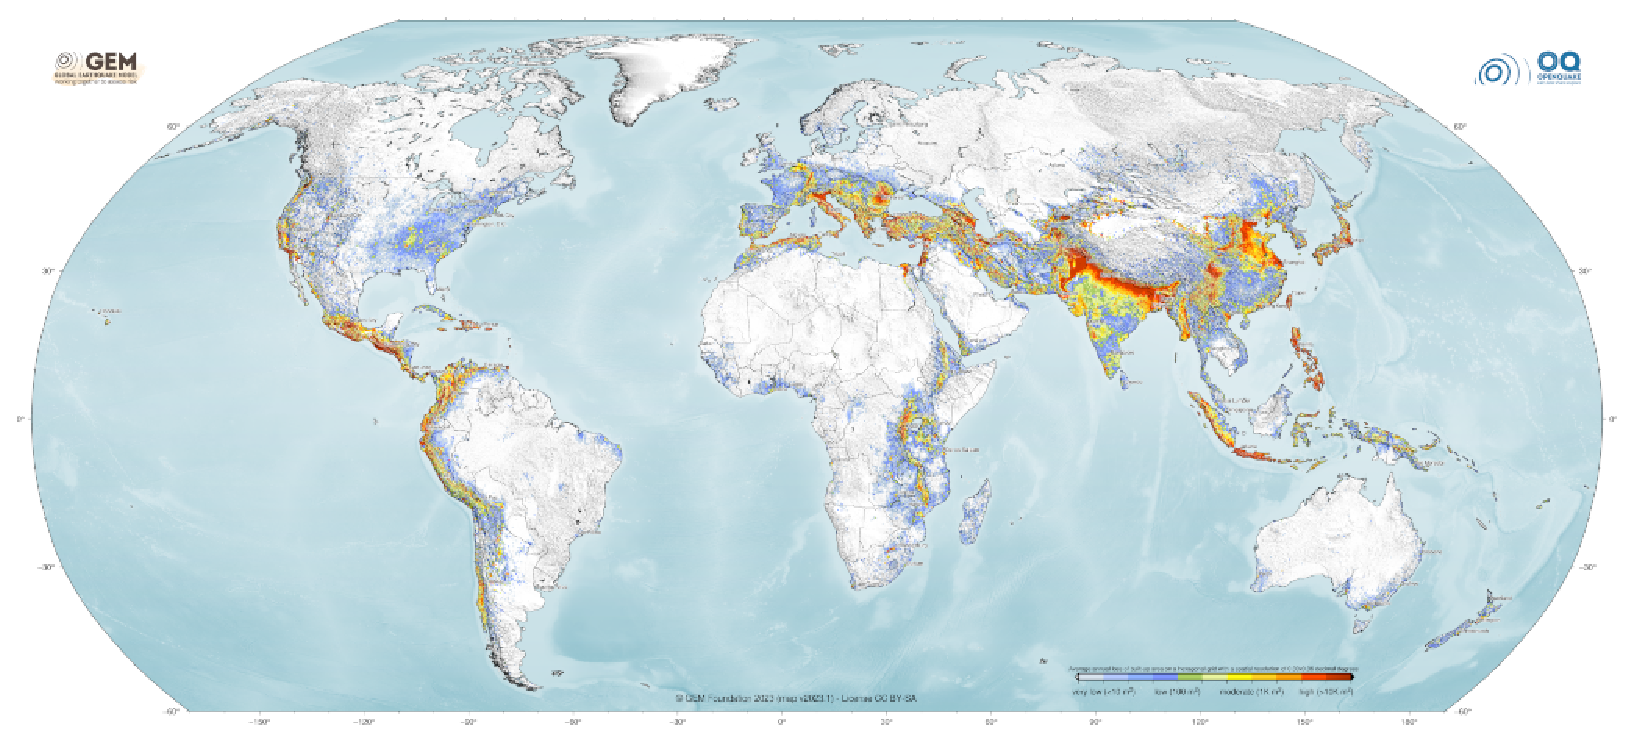
\includegraphics[scale=0.45]{gem_quake}
\par\end{centering}
\caption{Hazard map from Global Earthquake Model.\label{fig:Hazard-map-from}}

\end{figure}

In this framework, researchers are increasingly employing artificial
intelligence and other advanced methodologies to improve the timely
prediction of earthquakes and other natural hazards, aiming ultimately
to support communities in implementing protective actions and reducing
potential impacts\citep{Hutchinson2023}. A series of machine learning
techniques were applied on data gathered from earthquakes. For example,
Artificial neural networks (ANNs) \citep{nnoverview} were first applied
to the field of seismology in 1994, specifically through research
focused on earthquake prediction using seismic electric signals \citep{Lakkos1994}.
A more advanced form of an Artificial Neural Network (ANN) was employed
in the related study \citep{Mousavi2020}\textbf{. }Furthermore\textbf{,}
Mousavi et al. \citep{Mousavi2020-1} suggested an attentive deep-learning
model for simultaneous earthquake detection. Moreover, researchers
employed convolutional neural networks (CNNs)\citep{cnnSurvey} {[}11{]}
trained on over 18 million manually annotated seismograms from Southern
California to directly infer earthquake parameters from raw waveform
data, thereby eliminating the need for manual feature extraction.
The model demonstrated exceptional accuracy, achieving a standard
deviation of just 0.023 seconds in arrival-time estimation and a 95\%
success rate in polarity classification \citep{Ross2018}. 

The earliest application of Deep Neural Networks (DNNs) \citep{dnnOverview},
incorporating two hidden layers, was introduced in 2002 \citep{Negarestani2002}.
Subsequently, a high-resolution earthquake catalog was generated through
the application of deep neural network (DNN) techniques, providing
valuable insights into the complexity and temporal characteristics
of earthquake sequences, as well as their connections with recent
nearby seismic events, as outlined in related studies \citep{Tan2021}.
Additionally, Recurrent Neural Networks (RNNs) \citep{rnnOverview}
within the field of seismology was introduced in 2007 \citep{Panakat =000026 Adeli}.
Furthermore, a subsequent study regarding earthquake magnitude prediction
using machine learning techniques was introduced recently \citep{Asim et al.},
concentrated on forecasting earthquake magnitudes in the Hindukush
region. Four machine learning approaches neural network-based pattern
recognition, Recurrent Neural Networks, Random Forests \citep{rfOverview},
and a Linear Programming Boost ensemble classifier, were individually
applied to model the relationships between calculated seismic parameters
and the likelihood of future earthquake occurrences. Additionally,
a subsequent study showed that nearest-neighbor diagrams offer a straightforward
yet effective method for distinguishing between different seismic
patterns and evaluating the reliability of earthquake catalogs\citep{Hsu2024}.
Another research team, used Nearest Neighbor method, determined that
the Weibull model offered a more accurate fit for seismic data in
California, showing well-structured tail behavior. They further confirmed
the model’s robustness by successfully applying it to independent
datasets from Japan, Italy, and New Zealand, as reported in the related
publication \citep{Bayliss2019}. 

Building on recent advancements, Rouet‐Leduc et al. applied machine
learning techniques to datasets obtained from shear laboratory experiments,
with the objective of identifying previously undetected signals that
could potentially precede seismic events \citep{Rouet2017}. In a
subsequent study, the same research team applied a machine learning-based
method, initially developed in the laboratory, to analyze large volumes
of raw seismic data from Vancouver Island. This methodology enabled
the differentiation of pertinent seismic signals from background noise
and holds promise for evaluating whether, and under what conditions,
a slow slip event might be associated with or evolve into a major
earthquake \citep{Rouet2019}. Additionally, a recent study developed
a predictive model capable of estimating both the location and magnitude
of potential earthquakes for the following week. The model utilized
seismic data from the current week and targeted seismogenic regions
in southwestern China. It achieved a testing accuracy of 70\%, with
precision, recall, and F1 score values of 63.63\%, 93.33\%, and 75.66\%,
respectively. \citep{Saad2023}. Moreover, in another publication,
the research team demonstrated that machine learning techniques can
effectively predict the timing and magnitude of laboratory-induced
earthquakes by reconstructing and interpreting the system’s complex
spatiotemporal loading history \citep{Corbi2019}. 

Noteworthy, is the study by Zhang et al., which offers new perspectives
in the seismology field. Specifically, the authors succeeded in documenting
the directionality of coseismic acoustic waves generated by a major
earthquake, and in elucidating the coupling between seismic activity,
the ionosphere, and space weather. Their findings are presented in
the study titled “Successively equatorward propagating ionospheric
acoustic waves and possible mechanisms following the Mw7.5 earthquake
in Noto, Japan, on 1 January 2024”\citep{zhangQuake}. In contrast,
the current work focuses primarily on the classification of earthquakes
using Grammatical Evolution techniques. 

In this paper, a technique based on Grammatical Evolution \citep{mainGe}
is proposed for the efficient creation of classification rules on
seismic data that are widely available on the internet. Grammatical
Evolution is a genetic algorithm \citep{gaOverview}, where the chromosomes
are series of production rules from a provided Backus-Naur form (BNF)
grammar \citep{bnf1}. Among the numerous cases of application of
Grammatical Evolution, one can find problems such as\textbf{ }function
approximation\citep{ge_program1,ge_program2}, economic problems\citep{ge_credit},\textbf{
}network security issues \citep{ge_intrusion}, water quality problems
\citep{ge_water}, medical problems \citep{ge_glykemia}, evolutionary
computation \citep{ge_ant}, prediction of temperature in data centers
\citep{ge_datacenter}, solving trigonometric problems \citep{ge_trig},
composing music \citep{ge_music}, construction of neural networks
\citep{ge_nn,ge_nn2}, numerical problems \citep{ge_constant}, video
games \citep{ge_pacman,ge_supermario}, energy issues \citep{ge_energy},
combinatorial optimization \citep{ge_comb}, security issues \citep{ge_crypt},
evolution of decision trees \citep{ge_decision}, problems that appear
in electronics \citep{ge_analog} etc.

The main contributions of the current work are:
\begin{enumerate}
\item The proposed method investigates a wider geographical area than other
related studies, incorporating 255 seismic regions out of the 708
regions identified worldwide. 
\item The current work utilized a classification method based on Grammatical
Evolution to properly classify the seismic events in some predefined
classes. The use of this technique has two clear advantages: on the
one hand, it isolates those characteristics of a seismic event that
are deemed necessary for its effective classification and on the other
hand, it can discover, through the generation of complex rules, hidden
linear and nonlinear correlations between the characteristics of the
problem.
\end{enumerate}
The remainder of this paper is organized as follows: in section \ref{sec:Materials-and-Methods}
the used dataset is described as well as the steps of the proposed
method, in section \ref{sec:Results} the experimental results are
presented and finally in section \ref{sec:Conclusions} some conclusions
are discussed.

\section{Materials and Methods\label{sec:Materials-and-Methods}}

In this section, an extensive presentation of the seismic data used,
their post-processing, as well as the computational rule construction
method applied for the effective classification of earthquakes will
be given.

\subsection{The Dataset Employed}

In this study, we utilized open data provided by the NSF Seismological
Facility for the Earth Consortium (SAGE), specifically accessed through
the Interactive Earthquake Browser (\url{https://ds.iris.edu/}).
The choice of NSF data was motivated by its enhanced functionality.
The selection of NSF data was motivated by its high accessibility.
In particular, it allows for the download of up to 25,000 records
per file, substantially accelerating the workflow and enhancing information
retrieval. Additionally, the platform provides an interactive global
map, enabling both data visualization and the extraction of datasets
directly from the displayed geographical regions in real time. While
the GEOFON program offers comparable information, it limits the maximum
number of earthquakes retrievable per query to 1,000 events, thereby
constraining the temporal coverage of data extraction. This limitation
is especially relevant, as nearly 1,000 seismic events may occur globally
within a single day. The NSF SAGE Facility is acknowledged as a reliable
data repository, having been certified by the CoreTrustSeal Standards
and Certification Board.

\subsection{Dataset Description}

We downloaded and analyzed 1,035,971 earthquake events, from IEB,
between 2004-2011 (starting date 2004/04/01 - ending date 2011/03/16),
count days 2487. The dataset includes the following variables: Year,
Month, Day, Time, Latitude (Lat), Longitude (Lon), Depth, Mag, Region,
and Timestamp. We utilize the coordinates for (latitude 21°-79° \&
Longitude 33\textbf{°-}176°), select the magnitude measurements (range
1.0-10.0), and select by default for Depth Range, in order to use
all available depths. From our dataset, the daily average is 41,655
earthquakes; the minimum earthquakes in a day was 33, on 2005/03/02,
and the maximum in a day was 2326, on 2011/03/11 (Tohoku earthquake
9.1 mag). The regions encompassed within these geographical coordinates
are 255, while globally approximately 708 seismogenic zones have been
recorded since 1970, based on data from the Interactive Earthquake
Browser. The features of the original dataset are shown in Table \ref{tab:dataOriginal}.

\begin{table}[H]
\caption{The description of the original dataset.\label{tab:dataOriginal}}

\centering{}%
\begin{tabular}{|c|c|}
\hline 
FEATURE & RANGE\tabularnewline
\hline 
\hline 
YEAR & 2004-2011\tabularnewline
\hline 
MONTH & 1-12\tabularnewline
\hline 
DAY & 1-31\tabularnewline
\hline 
TIME & 00:00:00 - 23:59:59\tabularnewline
\hline 
LATITUDE & 21.00°-79.00°\tabularnewline
\hline 
LONGITUDE & 33.00°-176°\tabularnewline
\hline 
DEPTH & 0.00-800.00\tabularnewline
\hline 
MAGNITUDE & 1.0-10.0\tabularnewline
\hline 
TIMESTAMP & \tabularnewline
\hline 
\end{tabular}
\end{table}

We selected the specific time period for two main reasons. First,
it allowed us to manage the exceptionally large volume of seismic
data, amounting 1.035,971 records. Second, we observed a distinct
pattern in the seismic data from 2015 to 2025 that did not align with
established seismic trends. More specifically, the number of recorded
events rose to 46.400, a finding that prompted further consideration.
Regarding the geographical region, we deliberately selected seismic
zones with high activity, such as those in the Mediterranean including
Greece and Turkey, which share the same longitudinal range as Japan.

\subsection{Pre-processing steps}

The initial dataset was enhanced after processing the original data.
An important role in this process was played by the $d_{c}$ distance,
which will be used to determine when two earthquakes are close in
distance. This process attempts to include critical information about
seismic events that can potentially be extracted from seismic events
that are relatively close in both kilometer distance and time. Hence,
additional features were derived based on the critical distance $d_{c}$
to capture spatial-temporal proximity of events. The proposed value
in the present implementation was $d_{c}=$5 km. Based on the above
distance, the following features were added to the datasets:
\begin{enumerate}
\item Number of seismic events at a distance less than the $d_{c}$ that
have occurred in a previous time.
\item Average magnitude of seismic events at a distance less than $d_{c}$,
which have preceded the current seismic event in time.
\item The greatest magnitude of a seismic event recorded in the past, at
a distance of less than $d_{c}$ from the current seismic event.
\item The time in seconds since the largest seismic event that has occurred
in the past at a distance less than $d_{c}$ from the current seismic
event.
\item The distance in kilometers from the largest seismic event that has
occurred in the past at a distance less than $d_{c}$ from the current
seismic event.
\end{enumerate}
In addition, the size of the seismic recordings was divided into two
large classes:
\begin{itemize}
\item The first class contains all the events with magnitude $\le3$ 
\item The second class contains all the remaining events, with magnitude\textgreater 3.
\end{itemize}

\subsection{The used method}

The method that constructs classification rules was initially presented
in \citep{genclassMain} and an implementation in C++ was suggested
later by Anastasopoulos et al. \citep{genclassSoftx}. The method
can produce a series of classification rules in a human readable form
in order to effectively classify patterns in predefined classes. This
method does not require prior knowledge of the specifics of a dataset
and can furthermore discover hidden correlations between the features
of the dataset or even isolate only those features that play the most
significant role in the successful classification of patterns. The
method has been successfully applied in many cases, such as pollution
detection \citep{genClassPollution}, network problems \citep{genClassNetwork}
etc. The main steps of this method have as follows:
\begin{enumerate}
\item \textbf{Initialization step}.
\begin{enumerate}
\item \textbf{Set} the parameters of the genetic algorithm: $N_{c}$ as
the number of chromosomes, $N_{g}$ as the number of allowed generations,
$p_{s}$ as the selection rate and $p_{m}$ as the mutation rate.
\item \textbf{Perform} the initialization of chromosomes $g_{i},\ i=1,\ldots,N_{c}$.
Every chromosome is considered as a set of randomly selected integers. 
\item \textbf{Set} $k=0$, the generation counter.
\end{enumerate}
\item \textbf{Fitness calculation step}.
\begin{enumerate}
\item \textbf{For} $i=1,\ldots,N_{c}$ \textbf{do}
\begin{enumerate}
\item \textbf{Create} a classification program $C_{i}$ for the associated
chromosome $g_{i}$. The construction of this program is performed
using the BNF grammar of Figure \ref{fig:The-grammar-of}.
\item \textbf{The} produced classification program is applied to the train
set of the objective problem. Denote with $f_{i}$ (fitness value)
the classification error for this program. 
\end{enumerate}
\item \textbf{End For}
\end{enumerate}
\item \textbf{Application of genetic operations}.
\begin{enumerate}
\item \textbf{Selection}: The chromosomes are ranked according to their
fitness values. The $\left(1-p_{s}\right)\times N_{c}$chromosomes
with the lowest fitness are carried over to the next generation without
modification, while the remaining chromosomes are replaced by offspring
generated through crossover and mutation.
\item \textbf{Crossover}: In this procedure a series of offspring are produced,
through a process similar to biological crossover in nature. For every
couple $\left(\widetilde{z},\widehat{w}\right)$ of produced offsprings
two chromosomes are selected from the current population, using tournament
selection. Subsequently, these chromosomes will produce the set $\left(\widetilde{z},\widehat{w}\right)$
with the application of one-point crossover. A graphical example of
the one-point crossover method is outlined in Figure \ref{fig:onePoint}.
\item \textbf{Mutation}: During this procedure, a random number $r\in[0,1]$
is chosen for every element $g_{i,j}$ of each chromosome $g_{i}$.
Subsequently, this element is altered randomly when $r\le p_{m}$.
\end{enumerate}
\item \textbf{Termination check step}.
\begin{enumerate}
\item \textbf{Set} $k=k+1$
\item \textbf{If} $k\le N_{g}$ \textbf{then go to} Fitness Calculation
step \textbf{else} terminate.
\end{enumerate}
%
\end{enumerate}
\begin{figure}[H]
\begin{centering}
\includegraphics[scale=0.5]{genclass_grammar}
\par\end{centering}
\caption{The Backus-Naur form grammar used to generate classification rules
for seismic events.\label{fig:The-grammar-of}}

\end{figure}
\begin{figure}[H]
\begin{centering}
\includegraphics[scale=0.5]{cross2}
\par\end{centering}
\caption{An example of the one - point crossover method.\label{fig:onePoint}}

\end{figure}


\section{Experiments\label{sec:Results}}

The code employed in the experiments was implemented using the C++
programming language, along with the freely available optimization
tool \citep{optimus}, which can be downloaded from \url{https://github.com/itsoulos/GlobalOptimus.git}
(accessed on 12 October 2025). Additionally, the WEKA programming
tool \citep{weka_main} was utilized. C++ was chosen due to its high
computational efficiency. Each experiment was repeated 30 times, using
a different random seed for each run, and the average classification
error was reported. The experimental results were validated using
the ten-fold cross-validation method. The parameter values for the
employed methods are presented in \ref{tab:values}. 

\begin{table}[H]
\caption{The values for the experimental settings.\label{tab:values}}

\centering{}%
\begin{tabular}{|c|c|c|}
\hline 
PARAMETER & MEANING & VALUE\tabularnewline
\hline 
\hline 
$N_{c}$ & Chromosomes & 500\tabularnewline
\hline 
$N_{g}$ & Generations & 2000\tabularnewline
\hline 
$p_{s}$ & Selection rate & 0.1\tabularnewline
\hline 
$p_{m}$ & Mutation rate & 0.05\tabularnewline
\hline 
$d_{c}$ & Critical Distance & 5km\tabularnewline
\hline 
$H$  & Number of weights & 10\tabularnewline
\hline 
\end{tabular}
\end{table}


\subsection{Experimental results}

The following machine learning methods were used in the conducted
experiments as denoted in Table \ref{tab:Experimental-results}.
\begin{enumerate}
\item RBF, a Radial Basis Function (RBF) network \citep{rbf1,rbf2} was
incorporated with 10 weights.
\item MLP, an multilayer perceptron neural network \citep{nn1,nn2} with
10 processing nodes. The neural network was trained using the BFGS
optimization method \citep{powell}.
\item BAYES, where the Naive Bayes method \citep{naive_bayes} was utilized
on the dataset.
\item The column BAYESNN denotes the results from the application of the
Bayesian optimizer as implemented in BayesOpt \citep{bayesopt} library
to train a neural network with $H=10$ processing nodes. The code
can be downloaded from \url{https://github.com/rmcantin/bayesopt}
(accessed on 12 October 2025).
\item NNC, used to represent the application of Neural Network Construction
method \citep{nnc}, which creates the architecture of neural networks
using Grammatical Evolution.
\item GENCLASS, represents the application of the proposed method.
\end{enumerate}
\begin{table}[H]
\caption{Experimental results on the obtained datasets with the incorporation
of the mentioned machine learning methods. The acronyms are defined
as follows: RBF(Radial Basis Function networks), MLP (Multilayer Perceptron
Network), NNC (Neural Network Construction).\label{tab:Experimental-results}}

\centering{}%
\begin{tabular}{|c|c|c|c|c|c|c|}
\hline 
YEAR & RBF & MLP & BAYES & BAYESNN & NNC & GENCLASS\tabularnewline
\hline 
\hline 
2004 & 25.85\% & 26.55\% & 26.59\% & 28.23\% & 22.12\% & 18.92\%\tabularnewline
\hline 
2005 & 29.49\% & 28.10\% & 29.09\% & 28.73\% & 23.35\% & 19.56\%\tabularnewline
\hline 
2006 & 26.69\% & 27.67\% & 26.17\% & 25.50\% & 24.51\% & 17.19\%\tabularnewline
\hline 
2007 & 25.02\% & 26.93\% & 25.83\% & 24.89\% & 22.77\% & 18.14\%\tabularnewline
\hline 
2008 & 28.17\% & 29.97\% & 29.88\% & 28.53\% & 25.42\% & 19.51\%\tabularnewline
\hline 
2009 & 26.80\% & 25.90\% & 26.09\% & 25.08\% & 21.07\% & 17.81\%\tabularnewline
\hline 
2010 & 28.08\% & 29.43\% & 28.00\% & 26.22\% & 23.31\% & 19.89\%\tabularnewline
\hline 
2011 & 27.67\% & 35.83\% & 28.25\% & 28.56\% & 25.73\% & 20.97\%\tabularnewline
\hline 
AVERAGE & \textbf{27.22\%} & \textbf{28.80\%} & \textbf{27.49\%} & \textbf{26.97\%} & \textbf{23.54\%} & \textbf{19.00\%}\tabularnewline
\hline 
\end{tabular}
\end{table}
Also, the classification error for all methods per year is presented
in Figure \ref{fig:expYear}. 
\begin{figure}[H]
\begin{centering}
\includegraphics[scale=0.75]{quake_per_year}
\par\end{centering}
\caption{The classification error of each machine learning method per year.\label{fig:expYear}}

\end{figure}
Table \ref{tab:Experimental-results} reports yearly classification
error rates (2004-2011) for six machine-learning models. The proposed
GENCLASS method consistently ranks first every year, achieving the
lowest average error of 19.00\%, which corresponds to an overall accuracy
of about 81\%. The runner-up is NNC with an average error of 23.54\%,
so GENCLASS reduces error by roughly 4.54 percentage points on average,
about a 19\% relative reduction versus the closest competitor. The
annual margin of GENCLASS over NNC ranges from 3.20 to 7.32 points,
peaking in 2006. Beyond accuracy, GENCLASS also shows the smallest
across-year variability (standard deviation \ensuremath{\approx} 1.16),
indicating stable performance throughout the evaluation period. In
contrast, MLP exhibits the highest mean error (28.80\%) and the largest
variability, with a pronounced deterioration in 2011. Overall, these
results support the article’s claim that Grammatical Evolution is
particularly effective for this seismic classification problem, as
GENCLASS delivers both the lowest average error and the most consistent
year-to-year behavior.

The R-based significance analysis reveals a clear overall difference
among models (Friedman $p=1.21\times10^{-5}$, very strong evidence),
with pairwise tests indicating where these differences lie (Figure
\ref{fig:statClass}). GENCLASS outperforms MLP with $p=7.52\times10^{-4}$
(extremely significant) and BAYES with $p=0.00$6 (highly significant),
and the comparison with RBF is also statistically significant at $p=0.0125$.
In contrast, GENCLASS vs BAYESNN ($p=0.0516$) and GENCLASS vs NNC
($p=0.8937$) are not statistically significant at the $0.05$ threshold.
Overall, while the omnibus test confirms marked differences across
models, the superiority of the proposed method is clearly supported
against MLP, BAYES, and RBF, whereas the contrasts with BAYESNN and
NNC do not reach conventional significance.
\begin{figure}[H]
\includegraphics[scale=0.5]{stat_tbl4}

\caption{Statistical tests performed on the experimental results using the
variety of machine learning methods.\label{fig:statClass}}

\end{figure}


\subsection{Experiments with the critical distance $d_{c}$}

The critical distance $d_{c}$ was used to generate the final datasets
as the distance between seismic events. In order to determine the
correlation of this parameter with the experimental results produced,
another experiment was conducted where this distance ranged from 2
to 20km. In this experiment, the proposed classification rule generation
technique was used. The experimental results from this experiment
are presented in Table \ref{tab:dcExper}.The results indicate that
the critical distance $d_{c}$ influences performance, but the effect
size is small. The average classification error decreases slightly
as the distance increases: 19.08\% for $d_{c}=2km$, 19.00\% for 5km,
18.82\% for 10km, and 18.71\% for 20km. The gap between the worst
and best setting is 0.37 percentage points, i.e., about a 1.9\% relative
error reduction, so the overall advantage of the 20km setting is real
but modest. Year-by-year, $d_{c}=20km$ achieves the lowest error
in 4 out of 8 years (2004, 2005, 2009, 2010), $d_{c}=5km$ is best
in 2008, $d_{c}=10km$ in 2007, and $d_{c}=2km$, indicating no monotonic
or universally optimal choice across years but a mild preference toward
larger distances. Regarding stability, $d_{c}=2km$ shows the narrowest
range over time (17.51\%--20.70\%), whereas $d_{c}=20km$ exhibits
the largest spread mainly due to 2011 (16.97\%--21.78\%). Overall,
the method benefits marginally from increasing $d_{c}$, with 20km
yielding the lowest average error, but the choice should also consider
temporal stability and yearly idiosyncrasies, since the per-year optimum
shifts across settings.

\begin{table}[H]
\caption{Experiments with the GENCLASS method and different values of critical
distance $d_{c}$\label{tab:dcExper}}

\centering{}%
\begin{tabular}{|c|c|c|c|c|}
\hline 
YEAR & $d_{c}=2km$ & $d_{c}=5km$ & $d_{c}=10km$ & $d_{c}=20km$\tabularnewline
\hline 
\hline 
2004 & 18.69\% & 18.92\% & 18.54\% & 18.44\%\tabularnewline
\hline 
2005 & 18.47\% & 19.56\% & 18.26\% & 17.56\%\tabularnewline
\hline 
2006 & 17.51\% & 17.19\% & 17.38\% & 18.48\%\tabularnewline
\hline 
2007 & 20.03\% & 18.14\% & 18.06\% & 18.20\%\tabularnewline
\hline 
2008 & 20.70\% & 19.51\% & 20.69\% & 20.14\%\tabularnewline
\hline 
2009 & 17.90\% & 17.81\% & 17.39\% & 16.97\%\tabularnewline
\hline 
2010 & 19.21\% & 19.89\% & 19.32\% & 18.08\%\tabularnewline
\hline 
2011 & 20.09\% & 20.97\% & 20.91\% & 21.78\%\tabularnewline
\hline 
\textbf{AVERAGE} & \textbf{19.08\%} & \textbf{19.00\%} & \textbf{18.82\%} & \textbf{18.71\%}\tabularnewline
\hline 
\end{tabular}
\end{table}
The significance analysis across critical distance settings dc provides
no statistical evidence of an effect on classification error (Figure
\ref{fig:statDc}). The omnibus Friedman test is non-significant ($p=0.4153$),
indicating no systematic differences across $d_{c}$ levels. Pairwise
contrasts corroborate this: $d_{c}=2km$ vs 5km ($p=0.9803$), 10km
($p=0.5274$), and 20km ($p=0.5274$) are not significant, nor are
$d_{c}=5km$ vs 20km ($p=0.7675$) and $d_{c}=10km$ km vs 20km ($p=1$).
The $d_{c}=5km$ vs 10km comparison returned $p=\mbox{NA}$, which
typically reflects a degenerate post-hoc case (e.g., complete rank
ties or identical values per block) and does not alter the overall
conclusion. In sum, within the 2--20km range, dc does not yield statistically
significant performance differences for the proposed method, so this
hyperparameter may be selected based on practical or stability considerations
rather than expected accuracy gains.
\begin{figure}[H]
\includegraphics[scale=0.5]{stat_tbl5}

\caption{Statistical comparison for the results obtained by the application
of the GENCLASS method, using a variety of values for the critical
distance $d_{c}$.\label{fig:statDc}}

\end{figure}


\subsection{Experiments with the number of generations $N_{g}$}

An additional experiment was conducted to verify the stability of
the proposed classification rule generation technique. In this experiment,
the maximum number of generations ranged from 200 to 2000 and the
experimental results per year are presented in Table \ref{tab:ngExper}.
In this table, the results show a clear downward trend in classification
error as the maximum number of generations increases. The average
error decreases from 20.20\% $\left(N_{g}=200\right)$ to 19.58\%
$\left(N_{g}=500\right)$, 19.25\% $\left(N_{g}=1000\right)$ and
19.00\% $\left(N_{g}=2000\right)$, i.e., a total gain of 1.20 percentage
points or roughly a 6\% relative reduction compared to $N_{g}=200$.
Improvements exhibit diminishing returns: the largest drop is from
200 to 500 (\textminus 0.62), followed by 500 to 1000 (-0.33) and
1000 to 2000 (-0.25). On a per-year basis, $N_{g}=2000$ is best in
six out of eight years (2006-2011 except 2004-2005), while in 2004-2005
the minimum error occurs at $N_{g}=1000$. The 2005 value for $N_{g}=2000$
is noticeably higher than the other settings, which may reflect stochastic
variability or model over-specialization for that year’s data. The
spread across years is broadly similar across settings, so the main
benefit of increasing generations is a lower mean error rather than
a dramatic change in variability. In practice, the 1000-2000 range
offers the strongest performance, $N_{g}=1000$ comes very close to
$N_{g}=2000$ (0.25 points apart) and is attractive under tighter
computational budgets, whereas $N_{g}=2000$ yields the lowest average
error when runtime is not a constraint.

\begin{table}[H]
\caption{Experiments with the GENCLASS method and different values for the
number of generations $N_{g}$\label{tab:ngExper}}

\centering{}%
\begin{tabular}{|c|c|c|c|c|}
\hline 
YEAR & $N_{g}=200$ & $N_{g}=500$ & $N_{g}=1000$ & $N_{g}=2000$\tabularnewline
\hline 
\hline 
2004 & 19.85\% & 19.14\% & 18.76\% & 18.92\%\tabularnewline
\hline 
2005 & 17.94\% & 17.80\% & 17.63\% & 19.56\%\tabularnewline
\hline 
2006 & 20.33\% & 18.01\% & 17.95\% & 17.19\%\tabularnewline
\hline 
2007 & 20.51\% & 19.91\% & 19.37\% & 18.14\%\tabularnewline
\hline 
2008 & 21.83\% & 21.31\% & 20.16\% & 19.51\%\tabularnewline
\hline 
2009 & 18.61\% & 18.25\% & 18.15\% & 17.81\%\tabularnewline
\hline 
2010 & 20.59\% & 20.57\% & 20.55\% & 19.89\%\tabularnewline
\hline 
2011 & 21.90\% & 21.63\% & 21.39\% & 20.97\%\tabularnewline
\hline 
\textbf{AVERAGE} & \textbf{20.20\%} & \textbf{19.58\%} & \textbf{19.25\%} & \textbf{19.00\%}\tabularnewline
\hline 
\end{tabular}
\end{table}
The significance levels in Figure \ref{fig:statNg} indicate that
the maximum number of generations has an overall effect on performance,
as evidenced by a strongly significant Friedman test $\left(p=6.28\times10^{-4}\right)$.
In pairwise terms, moving from $N_{g}=200$ to $N_{g}=1000$ yields
a statistically significant error reduction ($p=0.022$), and the
contrast between $N_{g}=200$ and $N_{g}=2000$ is even more significant
($p=0.0067$), confirming that a low generation budget underperforms
relative to higher budgets. By contrast, $N_{g}=200$ vs $N_{g}=500$
is not significant ($p=0.8161$), nor are $N_{g}=500$ vs $N_{g}=2000$
($p=0.4306$) and $N_{g}=1000$ vs $N_{g}=2000$ ($p=0.9803$), suggesting
diminishing returns beyond roughly 1000 generations. The $N_{g}=500$
vs $N_{g}=1000$ comparison returned $p=\mbox{NA}$, typically due
to a degenerate post-hoc scenario (e.g., complete rank ties or identical
per-block values) and does not alter the main conclusion. Overall,
increasing generations above 200 significantly improves performance,
with gains saturating around 1000 generations and no clear statistical
advantage of 2000 over 1000.

\begin{figure}[H]
\includegraphics[scale=0.5]{stat_tbl6}

\caption{Statistical comparison for the results obtained by the usage of the
GENCLASS method, using different values for the maximum number of
generations $N_{g}$.\label{fig:statNg}}

\end{figure}


\section{Conclusions\label{sec:Conclusions}}

This study introduces an innovative methodology for earthquake classification
employing various machine learning methods, including RBF, MLP, BAYES,
NNC, along with the proposed GENCLASS approach. The analysis covers
seismic data recorded between 2004-2011, within the geographical bounds
of latitude 21°-79° and longitude 33°-176°. Our first process involved
classifying the size of the seismic events into two large classes:
The first class contains all the events with magnitude $\le3$. The
second class contains all the remaining events, with magnitude\textgreater 3,
followed by magnitude prediction based on the classified data. 

To construct the final datasets, the critical distance $d_{c}$ defined
as the distance between seismic events, was applied. The results indicate
that the proposed method benefits slightly from increasing $d_{c}$,
with a value of 20km yielding the optimal average error. Also we Set
as $N_{c}$ the number of chromosomes in the genetic population. Furthermore,
an additional experiment was conducted to evaluate the stability of
the proposed generations mechanism $N_{g}$. In this test, the maximum
number of generations was varied from 200-2000, indicating that the
maximum number of generations has an overall effect on performance.
Among all evaluated methods, GENCLASS consistently achieved the best
performance each year, attaining the lowest average error rate of
19\%, corresponding to an overall classification accuracy of 81\%. 

The main challenges encountered in this research were related to the
large volume of data, exceeding one million records, and the adaptation
of such data into a reliable classification system. In general, seismology
still keeps many of its secrets well guarded, but not indefinitely.
With the rapid advancement of machine learning and artificial intelligence
techniques, these mysteries are gradually being unraveled. Future
work in this area of research could include recent seismic events
as well as the use of other advanced computational intelligence techniques
such as feature construction from existing ones \citep{fcGE}. Furthermore,
since Grammatical Evolution is essentially a genetic algorithm, parallel
computing techniques can be used to speed up this process, such as
the OpenMP method \citep{openmp}or the OpenMPI programming library
\citep{openmpi}.

\vspace{6pt}


\authorcontributions{Conceptualization, C.K. and I.G.T.; methodology, C.K.; software,
I.G.T.; validation, C.S., V.C.; formal analysis, V.C.; investigation,
C.K.; resources, C.S.; data curation, C.K..; writing original draft
preparation, C.K.; writing review and editing, I.G.T.; visualization,
V.C.; supervision, C.S.; project administration, C.S.; funding acquisition,
C.S. All authors have read and agreed to the published version of
the manuscript.}

\funding{This research has been financed by the European Union : Next Generation
EU through the Program Greece 2.0 National Recovery and Resilience
Plan , under the call RESEARCH-CREATE-INNOVATE, project name “iCREW:
Intelligent small craft simulator for advanced crew training using
Virtual Reality techniques\textquotedbl{} (project code:TAEDK-06195).}

\institutionalreview{Not applicable.}

\informedconsent{Not applicable.}

\dataavailability{The original contributions presented in this study are included in
the article. Further inquiries can be directed to the corresponding
author.}

\conflictsofinterest{The authors declare no conflicts of interest.}


\appendix

\begin{adjustwidth}{-\extralength}{0cm}{}

\reftitle{References}
\begin{thebibliography}{99}
\bibitem[(2002)]{Mosegaard} Mosegaard, K., Tarantola, A., Lee, W.
H. K., Jennings, P., Kisslinger, C., \& Kanamori, H. (2002). International
Handbook of Earthquake and Engineering Seismology: Part A. International
Geophysics Series, 81, 237-265.

\bibitem[(2000)]{Richter-1}Online Archive of California, Guide to
the Papers of Charles F. Richter, 1839-1984. \url{https://oac.cdlib.org/findaid/ark:/13030/kt787005jn/admin/}

\bibitem[(2000)]{Mercalli-1} Encyclopedia.com, Mercalli, Giuseppe.
\url{https://www.encyclopedia.com/people/science-and-technology/environmental-studies-biographies/giuseppe-mercalli#:~:text=Mercalli}.

\bibitem[(2023)]{Geovera-1}GeoVera, A Journey Through Time: The History
of the Richter Scale, 2023. \url{https://geovera.com/2023/04/27/history-richter-scale/}

\bibitem{NAP-1}National Academies of Sciences, Engineering, and Medicine.
2003. Living on an Active Earth: Perspectives on Earthquake Science.
Washington, DC: The National Academies Press. \url{https://doi.org/10.17226/10493. https://nap.nationalacademies.org/read/10493/chapter/1#ii} 

\bibitem{Hutchinson2023}Hutchison, Allie. How machine learning might
unlock earthquake prediction. 2023. MIT Technology Review. \url{https://www.technologyreview.com/2023/12/29/1084699/machine-learning-earthquake-prediction-ai-artificial-intelligence/} 

\bibitem[(2008)]{nnoverview}Zou, J., Han, Y., \& So, S. S. (2008).
Overview of artificial neural networks. Artificial neural networks:
methods and applications, 14-22.

\bibitem{Lakkos1994}Lakkos, S., Hadjiprocopis, A., Comley, R., \&
Smith, P. (1994, September). A neural network scheme for earthquake
prediction based on the seismic electric signals. In Proceedings of
IEEE Workshop on Neural Networks for Signal Processing (pp. 681-689).
IEEE.

\bibitem{Mousavi2020}Mousavi, S. M., \& Beroza, G. C. (2020). A machine‐learning
approach for earthquake magnitude estimation. Geophysical Research
Letters, 47(1), e2019GL085976.

\bibitem{Mousavi2020-1}Mousavi, S. M., Ellsworth, W. L., Zhu, W.,
Chuang, L. Y., \& Beroza, G. C. (2020). Earthquake transformer---an
attentive deep-learning model for simultaneous earthquake detection
and phase picking. Nature communications, 11(1), 3952.

\bibitem[(2008)]{cnnSurvey}Li, Z., Liu, F., Yang, W., Peng, S., \&
Zhou, J. (2021). A survey of convolutional neural networks: analysis,
applications, and prospects. IEEE transactions on neural networks
and learning systems, 33(12), 6999-7019.

\bibitem{Ross2018}Ross, Z. E., Meier, M. A., \& Hauksson, E. (2018).
P wave arrival picking and first‐motion polarity determination with
deep learning. Journal of Geophysical Research: Solid Earth, 123(6),
5120-5129.

\bibitem[(2008)]{dnnOverview}Sze, V., Chen, Y. H., Yang, T. J., \&
Emer, J. S. (2017). Efficient processing of deep neural networks:
A tutorial and survey. Proceedings of the IEEE, 105(12), 2295-2329.

\bibitem{Negarestani2002}Negarestani, A., Setayeshi, S., Ghannadi-Maragheh,
M., \& Akashe, B. (2002). Layered neural networks based analysis of
radon concentration and environmental parameters in earthquake prediction.
Journal of environmental radioactivity, 62(3), 225-233.

\bibitem{Tan2021}Tan, Y. J., Waldhauser, F., Ellsworth, W. L., Zhang,
M., Zhu, W., Michele, M., ... \& Segou, M. (2021). Machine‐learning‐based
high‐resolution earthquake catalog reveals how complex fault structures
were activated during the 2016--2017 central Italy sequence. The
Seismic Record, 1(1), 11-19.

\bibitem[(2008)]{rnnOverview}Caterini, A. L., \& Chang, D. E. (2018).
Recurrent neural networks. In Deep neural networks in a mathematical
framework (pp. 59-79). Cham: Springer International Publishing.

\bibitem{Panakat =000026 Adeli}Panakkat, A., \& Adeli, H. (2007).
Neural network models for earthquake magnitude prediction using multiple
seismicity indicators. International journal of neural systems, 17(01),
13-33.

\bibitem{Asim et al.}Asim, K. M., Martínez-Álvarez, F., Basit, A.,
\& Iqbal, T. (2017). Earthquake magnitude prediction in Hindukush
region using machine learning techniques. Natural Hazards, 85(1),
471-486.

\bibitem[(2008)]{rfOverview}Breiman, L. (2001). Random forests. Machine
learning, 45(1), 5-32.

\bibitem{Hsu2024}Hsu, Y. F., Zaliapin, I., \& Ben‐Zion, Y. (2024).
Informative modes of seismicity in nearest‐neighbor earthquake proximities.
Journal of Geophysical Research: Solid Earth, 129(3), e2023JB027826.

\bibitem{Bayliss2019}Bayliss, K., Naylor, M., \& Main, I. G. (2019).
Probabilistic identification of earthquake clusters using rescaled
nearest neighbour distance networks. Geophysical Journal International,
217(1), 487-503.

\bibitem{Rouet2017}Rouet‐Leduc, B., Hulbert, C., Lubbers, N., Barros,
K., Humphreys, C. J., \& Johnson, P. A. (2017). Machine learning predicts
laboratory earthquakes. Geophysical Research Letters, 44(18), 9276-9282.

\bibitem{Rouet2019}Rouet-Leduc, B., Hulbert, C., \& Johnson, P. A.
(2019). Continuous chatter of the Cascadia subduction zone revealed
by machine learning. Nature Geoscience, 12(1), 75-79.

\bibitem{Saad2023}Saad, O. M., Chen, Y., Savvaidis, A., Fomel, S.,
Jiang, X., Huang, D., ... \& Chen, Y. (2023). Earthquake forecasting
using big data and artificial intelligence: A 30‐week real‐time case
study in China. Bulletin of the Seismological Society of America,
113(6), 2461-2478.

\bibitem{Corbi2019}Corbi, F., Sandri, L., Bedford, J., Funiciello,
F., Brizzi, S., Rosenau, M., \& Lallemand, S. (2019). Machine learning
can predict the timing and size of analog earthquakes. Geophysical
Research Letters, 46(3), 1303-1311.

\bibitem[(2024)]{zhangQuake}Zhang, B., Liu, T., Feng, X., \& Xu,
G. (2025). Successively equatorward propagating ionospheric acoustic
waves and possible mechanisms following the Mw 7.5 earthquake in Noto,
Japan, on 1 January 2024. Space Weather, 23(4), e2024SW003957.

\bibitem[(2002)]{mainGe}O'Neill, M., \& Ryan, C. (2002). Grammatical
evolution. IEEE Transactions on Evolutionary Computation, 5(4), 349-358.

\bibitem[(2017)]{gaOverview}Kramer, O. (2017). Genetic algorithms.
In Genetic algorithm essentials (pp. 11-19). Cham: Springer International
Publishing.

\bibitem[(2002)]{bnf1}J. W. Backus. The Syntax and Semantics of the
Proposed International Algebraic Language of the Zurich ACM-GAMM Conference.
Proceedings of the International Conference on Information Processing,
UNESCO, 1959, pp.125-132.

\bibitem{ge_program1}C. Ryan, J. Collins, M. O’Neill, Grammatical
evolution: Evolving programs for an arbitrary language. In: Banzhaf,
W., Poli, R., Schoenauer, M., Fogarty, T.C. (eds) Genetic Programming.
EuroGP 1998. Lecture Notes in Computer Science, vol 1391. Springer,
Berlin, Heidelberg, 1998.

\bibitem{ge_program2}M. O’Neill, M., C. Ryan, Evolving Multi-line
Compilable C Programs. In: Poli, R., Nordin, P., Langdon, W.B., Fogarty,
T.C. (eds) Genetic Programming. EuroGP 1999. Lecture Notes in Computer
Science, vol 1598. Springer, Berlin, Heidelberg, 1999.

\bibitem{ge_credit}A. Brabazon, M. O'Neill, Credit classification
using grammatical evolution, Informatica \textbf{30.3}, 2006.

\bibitem{ge_intrusion}S. Şen, J.A. Clark. A grammatical evolution
approach to intrusion detection on mobile ad hoc networks, In: Proceedings
of the second ACM conference on Wireless network security, 2009.

\bibitem{ge_water}L. Chen, C.H. Tan, S.J. Kao, T.S. Wang, Improvement
of remote monitoring on water quality in a subtropical reservoir by
incorporating grammatical evolution with parallel genetic algorithms
into satellite imagery, Water Research \textbf{ 42}, pp. 296-306,
2008.

\bibitem{ge_glykemia}J. I. Hidalgo, J. M. Colmenar, J.L. Risco-Martin,
A. Cuesta-Infante, E. Maqueda, M. Botella,J. A. Rubio, Modeling glycemia
in humans by means of Grammatical Evolution, Applied Soft Computing
\textbf{20}, pp. 40-53, 2014.

\bibitem{ge_ant}J. Tavares, F.B. Pereira, Automatic Design of Ant
Algorithms with Grammatical Evolution. In: Moraglio, A., Silva, S.,
Krawiec, K., Machado, P., Cotta, C. (eds) Genetic Programming. EuroGP
2012. Lecture Notes in Computer Science, vol 7244. Springer, Berlin,
Heidelberg, 2012.

\bibitem{ge_datacenter}M. Zapater, J.L. Risco-Martín, P. Arroba,
J.L. Ayala, J.M. Moya, R. Hermida, Runtime data center temperature
prediction using Grammatical Evolution techniques, Applied Soft Computing
\textbf{49}, pp. 94-107, 2016.

\bibitem{ge_trig}C. Ryan, M. O’Neill, J.J. Collins, Grammatical evolution:
Solving trigonometric identities, proceedings of Mendel. Vol. 98.
1998.

\bibitem{ge_music}A.O. Puente, R. S. Alfonso, M. A. Moreno, Automatic
composition of music by means of grammatical evolution, In: APL '02:
Proceedings of the 2002 conference on APL: array processing languages:
lore, problems, and applications July 2002 Pages 148--155. 

\bibitem{ge_nn}Lídio Mauro Limade Campo, R. Célio Limã Oliveira,Mauro
Roisenberg, Optimization of neural networks through grammatical evolution
and a genetic algorithm, Expert Systems with Applications \textbf{56},
pp. 368-384, 2016.

\bibitem{ge_nn2}K. Soltanian, A. Ebnenasir, M. Afsharchi, Modular
Grammatical Evolution for the Generation of Artificial Neural Networks,
Evolutionary Computation \textbf{30}, pp 291--327, 2022.

\bibitem{ge_constant}I. Dempsey, M.O' Neill, A. Brabazon, Constant
creation in grammatical evolution, International Journal of Innovative
Computing and Applications \textbf{1} , pp 23--38, 2007.

\bibitem{ge_pacman}E. Galván-López, J.M. Swafford, M. O’Neill, A.
Brabazon, Evolving a Ms. PacMan Controller Using Grammatical Evolution.
In: , et al. Applications of Evolutionary Computation. EvoApplications
2010. Lecture Notes in Computer Science, vol 6024. Springer, Berlin,
Heidelberg, 2010.

\bibitem{ge_supermario}N. Shaker, M. Nicolau, G. N. Yannakakis, J.
Togelius, M. O'Neill, Evolving levels for Super Mario Bros using grammatical
evolution, 2012 IEEE Conference on Computational Intelligence and
Games (CIG), 2012, pp. 304-31.

\bibitem{ge_energy}D. Martínez-Rodríguez, J. M. Colmenar, J. I. Hidalgo,
R.J. Villanueva Micó, S. Salcedo-Sanz, Particle swarm grammatical
evolution for energy demand estimation, Energy Science and Engineering
\textbf{8}, pp. 1068-1079, 2020.

\bibitem{ge_comb}N. R. Sabar, M. Ayob, G. Kendall, R. Qu, Grammatical
Evolution Hyper-Heuristic for Combinatorial Optimization Problems,
IEEE Transactions on Evolutionary Computation \textbf{17}, pp. 840-861,
2013.

\bibitem{ge_crypt}C. Ryan, M. Kshirsagar, G. Vaidya, G. et al. Design
of a cryptographically secure pseudo random number generator with
grammatical evolution. Sci Rep \textbf{12}, 8602, 2022.

\bibitem{ge_decision}P.J. Pereira, P. Cortez, R. Mendes, Multi-objective
Grammatical Evolution of Decision Trees for Mobile Marketing user
conversion prediction, Expert Systems with Applications \textbf{168},
114287, 2021.

\bibitem{ge_analog}F. Castejón, E.J. Carmona, Automatic design of
analog electronic circuits using grammatical evolution, Applied Soft
Computing \textbf{62}, pp. 1003-1018, 2018.

\bibitem[(2020)]{genclassMain}Tsoulos, I. G. (2020). Creating classification
rules using grammatical evolution. International Journal of Computational
Intelligence Studies, 9(1-2), 161-171.

\bibitem[(2020)]{genclassSoftx}Anastasopoulos, N.; Tsoulos, I.G.;
Tzallas, A. GenClass: A parallel tool for data classification based
on Grammatical Evolution. SoftwareX 2021, 16, 100830.

\bibitem[(2023)]{genClassPollution}Spyrou, E. D., Stylios, C., \&
Tsoulos, I. (2023). Classification of CO Environmental Parameter for
Air Pollution Monitoring with Grammatical Evolution. Algorithms, 16(6),
300.

\bibitem[(2023)]{genClassNetwork}Margariti, S. V., Tsoulos, I. G.,
Kiousi, E., \& Stergiou, E. (2024). Traffic Classification in Software-Defined
Networking Using Genetic Programming Tools. Future Internet, 16(9),
338.

\bibitem[(2025)]{optimus}I.G. Tsoulos, V. Charilogis, G. Kyrou, V.N.
Stavrou, A. Tzallas, Journal of Open Source Software \textbf{10},
7584, 2025.

\bibitem{weka_main}M. Hall, F. Frank, G. Holmes, B. Pfahringer, P.
Reutemann, I.H. Witten, The WEKA data mining software: an update.
ACM SIGKDD explorations newsletter \textbf{11}, pp. 10-18, 2009.

\bibitem[(1991)]{rbf1}J. Park and I. W. Sandberg, Universal Approximation
Using Radial-Basis-Function Networks, Neural Computation \textbf{3},
pp. 246-257, 1991.

\bibitem{rbf2}G.A. Montazer, D. Giveki, M. Karami, H. Rastegar, Radial
basis function neural networks: A review. Comput. Rev. J \textbf{1},
pp. 52-74, 2018.

\bibitem[(2018)]{nn1}Abiodun, O. I., Jantan, A., Omolara, A. E.,
Dada, K. V., Mohamed, N. A., \& Arshad, H. (2018). State-of-the-art
in artificial neural network applications: A survey. Heliyon, 4(11).

\bibitem{nn2}Suryadevara, S., \& Yanamala, A. K. Y. (2021). A Comprehensive
Overview of Artificial Neural Networks: Evolution, Architectures,
and Applications. Revista de Inteligencia Artificial en Medicina,
12(1), 51-76.

\bibitem{powell}M.J.D Powell, A Tolerant Algorithm for Linearly Constrained
Optimization Calculations, Mathematical Programming \textbf{45}, pp.
547-566, 1989. 

\bibitem{naive_bayes}G.I. Webb, E. Keogh, R. Miikkulainen, Naïve
Bayes, Encyclopedia of machine learning \textbf{15}, pp. 713-714,
2010.

\bibitem[(2014)]{bayesopt}Ruben Martinez-Cantin, BayesOpt: A Bayesian
Optimization Library for Nonlinear Optimization, Experimental Design
and Bandits. Journal of Machine Learning Research, 15(Nov):3735-{}-3739,
2014.

\bibitem{nnc}I.G. Tsoulos, D. Gavrilis, E. Glavas, Neural network
construction and training using grammatical evolution, Neurocomputing
\textbf{72}, pp. 269-277, 2008.

\bibitem[(2008)]{fcGE}Gavrilis, D., Tsoulos, I. G., \& Dermatas,
E. (2008). Selecting and constructing features using grammatical evolution.
Pattern Recognition Letters, 29(9), 1358-1365.

\bibitem[(2008)]{openmp}Chandra, R. (2001). Parallel programming
in OpenMP. Morgan kaufmann.

\bibitem[(2008)]{openmpi}Graham, R. L., Woodall, T. S., \& Squyres,
J. M. (2005, September). Open MPI: A flexible high performance MPI.
In International conference on parallel processing and applied mathematics
(pp. 228-239). Berlin, Heidelberg: Springer Berlin Heidelberg.

\end{thebibliography}
%%%%%%%%%%%%%%%%%%%%%%%%%%%%%%%%%%%%%%%%%%
%% for journal Sci
%\reviewreports{\\
%Reviewer 1 comments and authors' response\\
%Reviewer 2 comments and authors' response\\
%Reviewer 3 comments and authors' response
%}
%%%%%%%%%%%%%%%%%%%%%%%%%%%%%%%%%%%%%%%%%%

\PublishersNote{}

\end{adjustwidth}{}
\end{document}
